\section{Soluțiile problemelor}
\textbf{Seven Squares problema 1:}\newline\newline

\inputminted[linenos]{python}{code/ss1.out}

\newline
\begin{figure}[h]
    \centering
    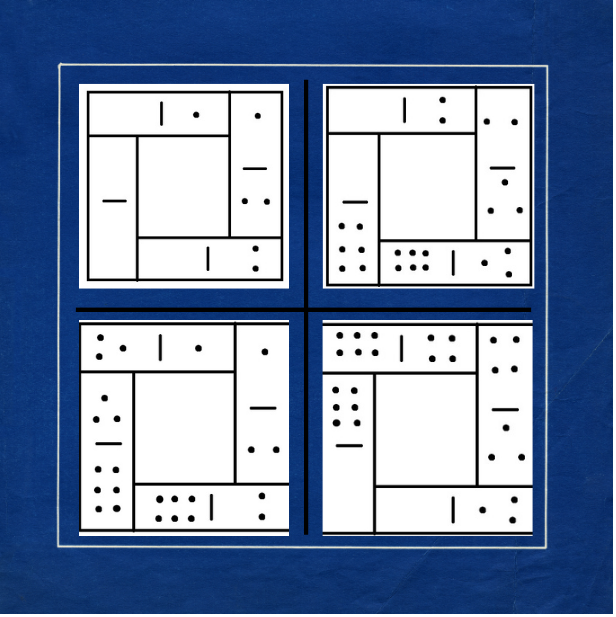
\includegraphics[width=12cm]{text/images/pic5.png}\\
    \caption{Seven Squares 1}
\end{figure} 
\newline\pagebreak

Am creat o vizualizare clară a celor 4 exemple alese random pentru prima problemă a dominourilor.
Se poate observa cu ușurință că se respectă cerințele problemei și că fiecare 2 vecini au aceleași numere.\pagebreak

\pagebreak
\newpage
\textbf{Seven Squares problema 2:}\newline\newline
\inputminted[linenos]{python}{code/ss2.out}\newline\newline\newline\newline\newline\newline\newline\newline
\newline\newline
\begin{figure}[h]
    \centering
    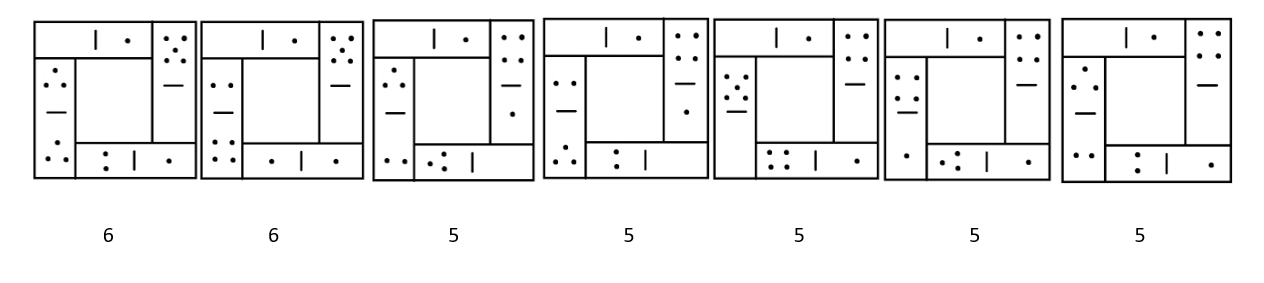
\includegraphics[width=16cm]{text/images/pic9.png}\\
    \caption{Seven Squares 2}
\end{figure} 
\newline\pagebreak


\textbf{The Resistance:}\newline\newline
\inputminted[linenos]{python}{code/spy.out}

